\documentclass[11pt]{article}
\usepackage[a4paper, portrait, margin=1in]{geometry}
\usepackage{graphicx}
\usepackage{url}


\begin{document}

\title{Advanced Systems Lab (Fall'15) -- First
Milestone}

\author{Name: \emph{Marcel Mohler}\\Legi number: \emph{09-922-998}}

\date{
\vspace{4cm}
\textbf{Grading} \\
\begin{tabular}{|c|c|}
\hline  \textbf{Section} & \textbf{Points} \\ 
\hline  1.1 &  \\ 
\hline  1.2 &  \\ 
\hline  1.3 &  \\ 
\hline  2.1 &  \\ 
\hline  2.2 &  \\ 
\hline  2.3 &  \\ 
\hline  3.1 &  \\ 
\hline  3.2 &  \\ 
\hline  3.3 &  \\ 
\hline  3.4 &  \\ 
\hline  3.5 &  \\ 
\hline  3.6 &  \\ 
\hline \hline Total & \\
\hline 
\end{tabular} 
}

\maketitle

\newpage

\section{System Description}\label{sec:system-description}
This report describes the implementation and performance of a message passing system called \textbf{SimpleMQ}.
\subsection{Database}\label{sec:database}

\subsubsection{Schema and Indexes}\label{sec:schema-and-indexes}
Our goal was to keep the database schema as simple as possible to avoid the need of complex queries. In the absence of costly table join operations, we hope to achieve a more predictable database performance without the need to worry about manually optimizing our queries. The layout is depicted in Figure \ref{fig:dbschema}. We use a single table to store all the messages and two more tables for the clients and queues. The ids of \texttt{queues} and \texttt{clients} pose a foreign key constraint to the \texttt{messages} table. This means that it is not possible to insert a message with a sender, receiver or queue id that does not exist in the database without the database throwing an error.\\
Since we want to be able to efficiently delete clients and queues we created an index on id in both \texttt{clients} and \texttt{queues}.
On the \texttt{messages} table indexes on id (\texttt{pop\_queue()}), queue\_id (\texttt{pop\_queue()}, \texttt{peek\_queue()}), sender\_id (\texttt{pop\_message()}) and receiver\_id (\texttt{pop\_queue()}, \\\texttt{peek\_queue()}, \texttt{pop\_message()}) were created to allow performant selection on these columns. The brackets denote the queries that profit from these indexes which are described in more detail in section \ref{sec:stored-procedures}.
\begin{figure}[ht!]
  \begin{center}
    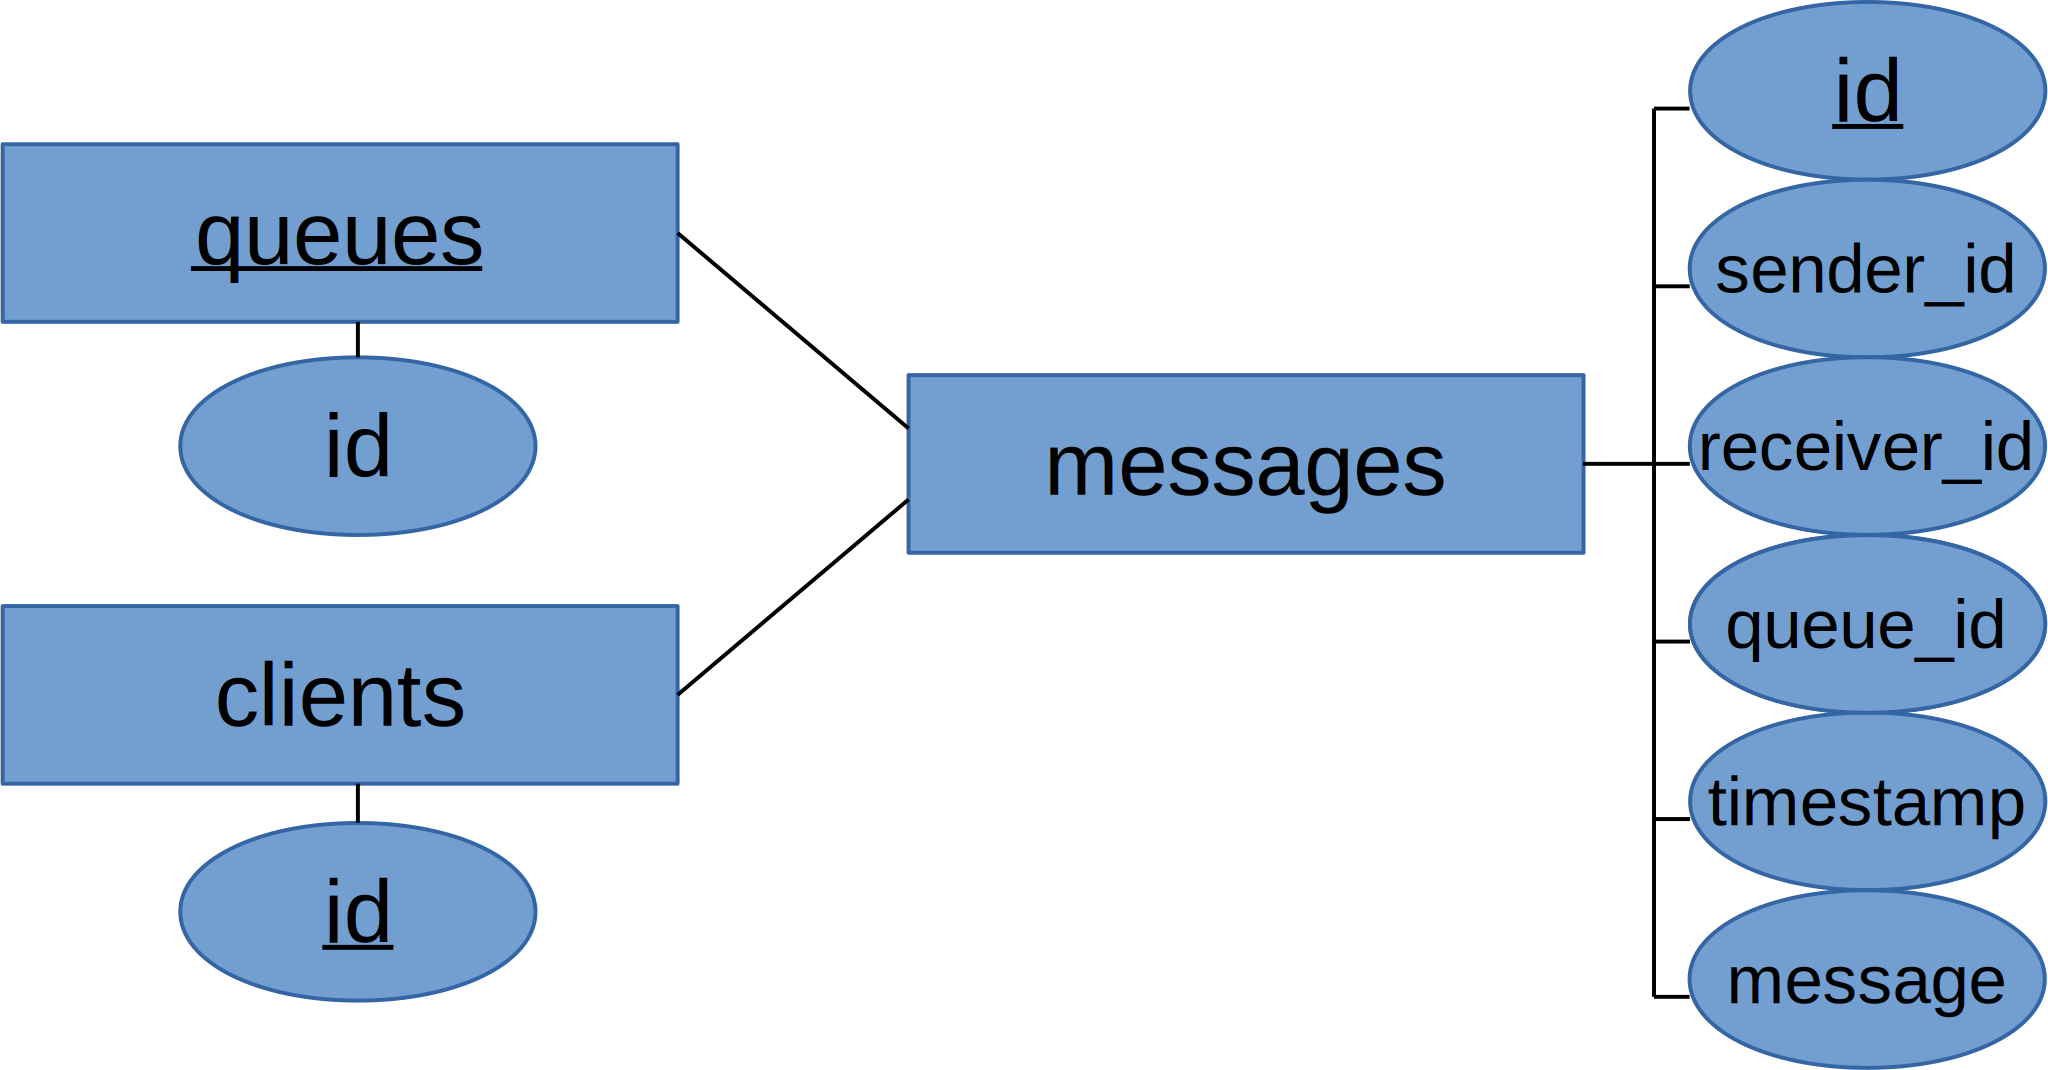
\includegraphics[width=0.6\textwidth]{figures/dbschema.pdf}
    \caption{DB schema}
    \label{fig:dbschema}
  \end{center}
\end{figure}

\subsubsection{Stored Procedures}\label{sec:stored-procedures}
Table \ref{tab:storedprocedures} describes the stored procedures used in SimpleMQ. The arguments client, sender, receiver, queue denote a particular client or queue id.
\\If the return column is denoted by \textit{auto-inc}, this means that the returned ID is automatically incremented by the database.
\\Because we assume in our workloads, that clients know about each other and experiments are designed such that each client has a unique ID, we allow the \texttt{add\_client} procedure to receive an ID as parameter. This is an intentional simplification to allow easier tracking of the clients when we later evaluate the system's performance.
\begin{table}[ht]
  \caption{stored procedures in SimpleMQ}
  \label{tab:storedprocedures}
  \begin{center}
    \begin{tabular}{|p{5cm}|p{6cm}|p{1.8cm}|}
       \hline
       \textbf{stored procedure name} & \textbf{description} & \textbf{returns}\\ \hline
       \texttt{add\_message}(sender, receiver, queue, timestamp, message) & adds a new message & msg\_id auto-inc\\ \hline
       \texttt{add\_queue}() & adds a new queue & queue\_id auto-inc\\ \hline
       \texttt{delete\_queue}(queue) & deletes the queue & nothing\\ \hline
       \texttt{query\_queues}(client) & queries for a queue where messages for the client are waiting & queue\_id\\ \hline
       \texttt{add\_client}(client) & add a new client & nothing\\ \hline
       \texttt{delete\_client}(client) & deletes the client & nothing\\ \hline
       \texttt{pop\_message}(sender, receiver) & reads and removes the oldest message from a particular sender & message\\ \hline
       \texttt{pop\_queue}(queue, receiver) & reads and removes the oldest message for a particular receiver & message\\ \hline
       \texttt{peek\_queue}(queue, receiver) & reads the oldest message for a particular receiver & message\\ \hline
    \end{tabular}
  \end{center}
\end{table}
\subsubsection{Design decisions}\label{sec:design-decisions}
While the simplicity of the schema favors the ability to write uncomplex queries, we expect this to have an negative influence on performance.
In particular, apart from clients and queue creation/deletion, all queries operate on the single table \texttt{messages}. This means that when multiple middlewares access the database concurrently, the database has to deploy locking mechanisms to prevent concurrency artifacts like dirty reads, lost updates or phantoms\footnote{see ETH Lecture Inf. Systems: \url{https://globis.ethz.ch/files/2015/04/IS-lect14-concurrency.pdf}}. PostgreSQL guarantees the absence of these artifacts, but the mechanisms that prevent this will have an impact on the database performance, particularly increase the response time on concurrent access. 
\subsubsection{Performance characteristics}\label{sec:performance-characteristics}
\textbf{Decription:}\\
To measure baseline performance of the database, we run the system in a special way, where the clients contact the database directly and no middleware server is used. The clients simply issue requests with no think time in between and keep an own connection to the database each.\\
We use a single \textit{AWS EC2 M4} instance for the database (the same as in later experiments) and two of these instances for the clients.\\
We scale the clients from 10 to 100 and draw the throughput and response time in Figure \ref{fig:dbonly}.\\
\begin{figure}
  \begin{center}
    \includegraphics[width=0.8\textwidth]{../results/dbonly.pdf}
    \caption{Database baseline performance with small and large messages}
    \label{fig:dbonly}
  \end{center}
\end{figure}
\textbf{Hypothesis:}\\
We expect the throughput to increase until a certain number of clients is reached. This is when the database handles as many requests per second as possible (saturation). At the same time, we expect the response time to increase, because the more clients the more parallel accesses to the database are required and the database potentionally has to wait longer for a (partial) lock on the table.\\
\textbf{Explanation:}\\
For small messages, we can see, that the throughput in (a) approaches a maximum of 1950 messages/second at 80 clients. When using large messages, the database can not handle more than 1429 messages/second at 60 clients. Large messages are 10x larger than small ones which means they take longer to store and retreive from the database which explains the performance differences.

\subsection{Middleware}\label{sec:middleware}
Length: 1-2 pages

Explain the design from a high-level point of view, highlighting what
you wanted to achieve, design decisions, expected behavior.

Then go into more detail on how the middleware connects to the database
and clients, and how queuing is implemented.

Show what are the performance characteristics of the middleware
(i.e.~throughput, latency, scalability).

\subsubsection{Design overview}\label{sec:design-overview}
The main goal was to provide a middleware, that scales well, when increasing the number of clients. This means that we expect the system throughput to r constant once the middleware receives the maximum number of requests it can support. This quantity is determined by the amount of internal worker threads which is equal to the amount of possible connections to the database.
Adding more clients to the system should not negatively impact performance but at the same time no clients should suffer from starvation.
\\
To allow asynchronous requests we have chosen to implement the middleware using Java NIO.
\\
Each middleware instance basically consists of two major components: one distributor and multiple worker threads.
The distributor iterates over incoming requests (also called \textit{key} in Java NIO) and distributes these requests to the workers. Available workers are stored in a concurrent blocking queue. This means that in case no worker is available, the distributor will wait until a worker finishes. The total amount of workers is a configurable parameter.

\begin{figure}[ht!]
  \begin{center}
    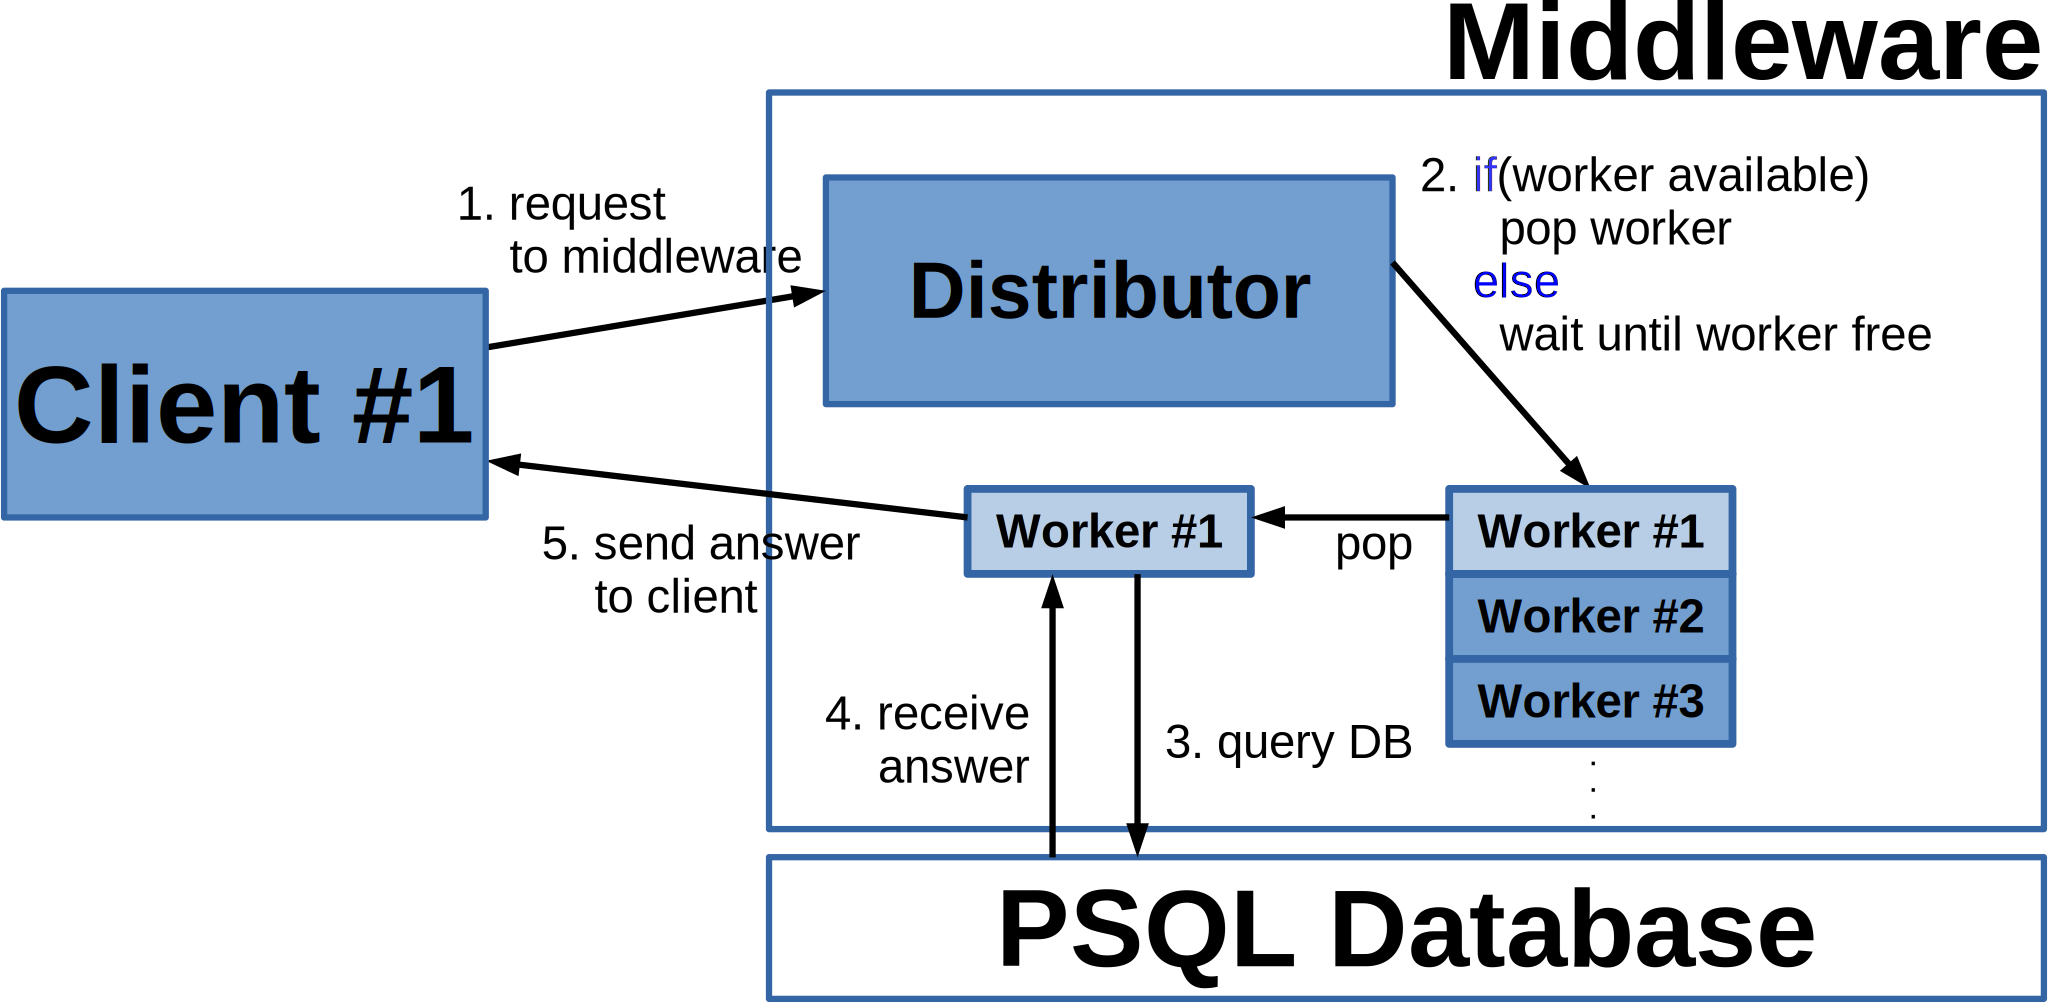
\includegraphics[width=0.8\textwidth]{figures/middleware.pdf}
    \caption{Overview of the system}
    \label{fig:middleware}
  \end{center}
\end{figure}

\subsubsection{Interfacing with clients}\label{sec:interfacing-with-clients}
The middleware provides a ServerSocket on a predefined port. Clients can send requests to that port and the server will handle them eventually (asynchronously).
Clients need to start by issueing a \texttt{CreateClient} request. The middleware then contacts the database to insert the clients ID. As soon as a client sends a \texttt{DeleteClient} request, the middleware deletes its ID from the database.
The requests and answers are serialized Java classes, defined in a shared API.

\subsubsection{Queuing and Connection pool to database}\label{sec:queuing-and-connection-pool-to-database}
Every worker maintains a persistent connection to the database. In our experiments we always make sure that we do not have more workers than the amount of simultaneous connections the database accepts.
\subsubsection{Performance characteristics}\label{sec:performance-characteristics-1}
todo

\subsection{Clients}\label{sec:clients}

Length: 2-3 pages

Explain the interface of the clients to your messaging system and their
high level design, including the ways you have instrumented the code for
debugging and benchmarking purposes.

Provide a detailed description of the workloads used later in the report
(operation mix, starting and ending state of the database, assumptions
on workload behavior). Explain how the load was generated (include
baselines on load generation speed) and how the clients were deployed.

Which are the sanity checks in place for ensuring correct load
generation and validity of responses?

\subsubsection{Design and interface}\label{sec:design-and-interface}
The clients are designed as simple as possible. They basically consist of a while loop, that sends messages until either the maximum number of messages or a timelimit is reached. Both are configurable parameters.
We also allow an additional wait time to be added in between receiving an answer and sending the next request (called think time).
The baseline performances were measured using AWS EC2 M4 instances by measuring the time it takes to create the objects and put on the output stream.
\subsubsection{Instrumentation}\label{sec:instrumentation}
Each client keeps a log of all outgoing requests and incoming answers.
The logs contain a timestamp a unique request ID and information about the message type. Logged answers also include the measured time since sending the message and receiving the answer (response time).\\
The unique ID is used to check whether the received answer belongs to the sent request. However, this should always be the case in our closed loop system.
\subsubsection{Workloads and deployment}\label{sec:workloads-and-deployment}
The client has an abstract class \texttt{TrafficGenerator}. We use this to be able to simply implement different TrafficGenerators that resemble different workloads. We present the implementations relevant to the measurements:
\begin{itemize}
  \item \textbf{staticsmall}: This denotes a workload, where the client sends one of the following three requests iteratively: SendMessageToQueue, PeekMessageFromQueue, PopMessageFromQueue.\\
  In this workload, we only use a single queue with ID 1.
  It sends it's messages to the client with the own client id incremented by one (and a wrap around to 1 for the client with the largest ID).
  Because the amount of messages send to the system (using SendMessageToQueue) and deleted from the system (using PopMessageFromQueue) are the same, the number of messages in the database should remain constant.
  However, due to different start times of the clients it can happen that a pop does not return any message. In this case, the client will log this incident and the message will not be included in performance measurements. The clients will not repeat these unsuccessful pops or peeks, but since SendMessage usually succeed, after some warmup, the database will always contain a few messages and these errors get fewer.
  In \textbf{staticsmall}, the message payload is a constant string of 200 characters.\\
  A client using this workload can create TODO small messages per second on average.
  \item \textbf{staticlarge}: This is the same as \textbf{staticsmall} but the message payload got increased to 2000 characters.\\
  A staticlarge client can generate  TODO large messages per second.
\end{itemize}
Except for the 30 minute run, the database starts empty. As mentioned before, since the in and output is constant the database will usually contain close to zero messages.

\subsubsection{Sanity checks}\label{sec:sanity-checks}
The clients are designed as a closed loop system. They only issue the next request when they have received the previous answer. The client also checks the message integrity before it logs a succesful attempt. If the message content is unexpected, e.g. an answer message ID does not match the request message ID or the payload got corrupted, we log this error and do not count these messages towards the total throughput.
\section{Experimental Setup}\label{sec:experimental-setup}

Length: 1-2 pages

Explain the overall design of the complete system and list the
configurations (number of middlewares, number of clients, types of
machines, communication patterns) corresponding to the main workloads.

Describe the mechanisms for deploying the system for experiments and the
way performance numbers are gathered and processed. Make the description
so that someone unfamiliar with your system can replicate the steps, and
reference the different script files you submit as code in the SVN
repository.

\subsection{System Configurations}\label{sec:system-configurations}
To deploy the clients, middleware and database we always use the \textit{Amazon AWS EC2 M4} instances. They offer two virtualized CPU cores, 8GB of main memory and are configured to use 8 GB of SSD storage and run Ubuntu Server 14.04 LTS.\\
We chose this instance type since it provides us with stable CPU performance (compared to the CPU burst capability of the \textit{AWS EC2 T2} instances), while still remain a relatively low price so we have enough funds to do all the measurements.
A comment on the Amazon AWS services:
Initially, AWS caused us a lot of trouble to achieve consistent results. One of the main reasons was the usage of \textit{AWS EC2 T2 instances}. They are called Burstable Performance Instances and provide a baseline performance and the ability to boost performance using CPU credits. The CPU credits reload at a specific rate. However, the fact that it is very hard to track the current status of these CPU credits and made it very hard to compare individual measurements. An experiment using available CPU runs significantly faster than experiments when no more CPU credits are available.\\
Therefore we decided to use \textit{AWS EC2 M4} instances which should provide a fixed CPU performance.
\subsection{Configuration and Deployment mechanisms}\label{sec:configuration-and-deployment-mechanisms}
We tried to automate the deployment mechanisms as much as possible. Several scripts were written to achieve this goal.
\begin{itemize}
  \item \texttt{experiment.sh:} This script makes sure all instances are running the latest versions, runs the benchmarks and gathers the results. It runs locally and uses amazon instance IP's as arguments. In particular the steps are: \\1. parse command line parameter \\2. build server and client from source into a .jar using \texttt{ant}\footnote{\url{https://ant.apache.org/}} \\3. check if passwordless login is enabled \\4. cleanup servers in case some old experiments are still running \\5. copy compiled .jar's to client and server instances \\6. setup postgres \\7. run database, server and clients remotely \\8. wait for the clients to finish \\9. shutdown database and server \\10. copy log files from remote locations \\11. invoke further processing of log files
  \item \texttt{client.sh:} Helper script to run individual clients on the client instances. This prevents the need of keeping alive a connection to each individual client. This will be copied to the client machines and invoked automatically.
\end{itemize}
\subsection{Logging and Benchmarking mechanisms}\label{sec:logging-and-benchmarking-mechanisms}
\begin{itemize}
  \item \texttt{graphs.py:} This Python program parses the merged log files of the clients and provides metrics like throughput per second, response time and several statistical properties of the data. It also uses matplotlib to provide throughput and response time over time graphs.
  \item \texttt{graphs\_server.py:} This is very similar to \texttt{graphs.py} but parses the server log files instead.
  \item \texttt{evalThroughputResponse.py:} After the logs have been parsed by previous scripts, this script parses the output and provides .csv files to use with the plotting tool veusz\footnote{\url{http://home.gna.org/veusz/}}.
 \end{itemize}

\section{Evaluation}\label{sec:evaluation}

Length: up to 10 pages

In this section we expect to see the different experiments you ran to
exercise the system, and with each experiment we expect a clear
description of the system configuration used, the hypothesis on behavior
and the explanation of the behavior observed (in terms of the different
design decisions taken beforehand) -- \emph{missing either of these for
an experiment might make you lose all points for that given experiment!}
Keep in mind that for a good explanation of the results of an experiment
you might have to use one or more methods of data analysis presented in
the lecture and in the book.

See below for a short description on what each part should contain.

\subsection{System Stability}\label{sec:system-stability}

% To prove that your system functions correctly and that it is stable
% include the trace of a 30 minute run, plotting both response time and
% throughput. Use at least 30 clients (sending and receiving data), 2
% middlewares and a non-empty database.
\textbf{Decription:}\\
To show the stability of the system we let the system running for 1980 seconds (33 minutes). We use 30 clients on a single instance and two middleware servers with 32 workers each. The database is preloaded with 5000 messages.\\
We use a think time of 0 seconds on the clients.
We cut out the first minute to eliminate warmup effects.
The trace of the throughput and the response time over time for message sizes small and large is shown in Figure \ref{fig:longrun}.\\
\begin{figure}[ht!]
  \begin{center}
    \includegraphics[width=0.8\textwidth]{../results/longrun.pdf}
    \caption{}
    \label{fig:longrun}
  \end{center}
\end{figure}
\textbf{Hypothesis:}\\

\textbf{Explanation:}\\


\subsection{System Throughput}\label{sec:system-throughput}
\textbf{Decription:}\\
In Subsection \ref{sec:performance-characteristics} we analyzed the baseline performance of the database. Using our defined workload staticsmall (see \ref{sec:workloads-and-deployment}, we saw, that our database can not handle more than approximately 1950 messages per second. This imposes an upper bound on what we can achieve in this experiment because we can not further increase the database performance without changing the schema or the workload. We keep the previously defined workload, because the balanced send and receive operations reflect a realistic usage scenario of a message passing system.\\
Our aim for the system throughput is to get as close to the database baseline performance as possible.\\
For this experiment we consider the full system again. We use 3 instances for the clients and 2 middlewares to make sure the instance performance is not limiting.\\
In case the clients combined message generation is higher than the throughput the middleware can handle, message requests are queued at the distributor layer of the middleware. In this case, as soon as a worker has finished a request he has to handle the next one and is never idle. \\
Because we measured, that the DB baseline maximum throughput was generated using 80 clients sending with 0 think time we start by trying to achieve the peak system throughput with 80 middleware workers.\\
We now need to make sure, that the middleware is actually receiving enough requests and workers are not idle. Because of network delay and compute overhead at the clients and middleware we need more clients than worker threads to achieve this goal.\\
We start with 100 workers and 80 clients and will then continue varying these two parameters and observe the impact on throughput and response time.\\

\begin{table}
  \caption{}
  \begin{center}
    \begin{tabular}{ r|c|c|c|c|c| }
    \multicolumn{1}{r}{}
     & \multicolumn{1}{c}{54 clients}
     & \multicolumn{1}{c}{60 clients}
     & \multicolumn{1}{c}{66 clients}
     & \multicolumn{1}{c}{100 clients}
     & \multicolumn{1}{c}{140 clients} \\
    \cline{2-6}
    60 workers & & 1845.4+-146.7 & & 1507.3+-253.0
& 977.2+-46.4\\     
    \cline{2-6}
    80 workers & & 1849.0+-78.1 & 
& 1591.1+-117.0
&1041.7+-17.1
\\
    \cline{2-6}
    100 workers & & 1840.7+-204.0 &
& 1531.1+-306.6
&1021.8+-64.7
\\
    \cline{2-6}
    \end{tabular}
  \end{center}
    \label{tab:}
\end{table}
\textbf{Hypothesis:}\\

\textbf{Explanation:}\\
Measure the maximum throughput of the system (describe the exact
configuration and workload, and the reasoning behind choosing these
particular ones) and show the average response time for this experiment.

\subsection{System Scalability}\label{sec:system-scalability}

We start by doing the following two experiments:
\begin{enumerate}
  \item Fix the number of workers and scale the clients
  \item Fix the number of clients and scale the workers
\end{enumerate}
We expect these experiment to give us evidence how the system behaves when we increase either resource, but limit the other. Detailed hypotheses are provided on each experiment individually below.
We also use a client think time of 0. While this does not reflect any real life scenario it allows us to use as few clients as possible that generate as many messages as they can.
\subsubsection{Fix workers - scale clients}
\textbf{Decription:}\\
We use two middleware node (AWS M4) with a fixed number of 30 concurrent workers each. We scale the amount of clients from 5 to 100 in steps of 5-10. For each number of clients we run the system for 300 seconds and repeat it three times to be able to provide empirical evidence.\\
\textbf{Hypothesis:}\\
We limit the amount of workers on the system, so the throughput is also limited. That is, because if all workers are constantly busy no additional messages can be handled and will therefore only be processed once a worker is free again. \\
As one can see in Figure \ref{fig:maxclientperinstance} (a), we expect the throughput to rise linearly until a certain threshold and then keep that level. This threshold is the saturated state of the system. Since we use no think time and clients can serve new messages very quickly we assume this threshold being somewhere, where number of clients matches number of middleware workers. This hypothesis is based on the fact that delay of sending messages between client and middleware is far less than the delay between middleware and database (see ref TODO).
\textbf{Explanation:}\\

\begin{figure}[ht]
  \begin{center}
    \includegraphics[width=0.9\textwidth]{../results/maxclientperinstance.pdf}
    \caption{Scaling the number of clients - left small, right large messages}
    \label{fig:maxclientperinstance}
  \end{center}
\end{figure}
\subsubsection{Fix clients - scale workers}
\textbf{Decription:}\\
Analog to the previous experiment, we now fix the number of clients to 60. We use 2 AWS M4 nodes to run these clients.\\
Now we scale the number of workers from 10 to 100 in steps of 10 and keep the rest of the setup in terms of time and repetitions.\\
\textbf{Hypothesis:}\\
\textbf{Explanation:}\\
\begin{figure}[ht]
  \begin{center}
    \includegraphics[width=0.9\textwidth]{../results/maxworkerperinstance.pdf}
    \caption{Scaling the number of workers - left small, right large messages}
    \label{fig:maxworkerperinstance}
  \end{center}
\end{figure}
Explain the different configurations used to explore the scalability of
your system, and the outcomes of these experiments in terms of
throughput and response times. The main goal of this subsection is to
define the ranges in which your system operates best.

\subsection{Response Time Variations}\label{sec:response-time-variations}

Report and analyze how the response times change in the system with
different message sizes, different number of clients and different
number of middleware nodes.

\subsection{$2^k$ Experiment}\label{sec:k-experiment}
\begin{table}
  \caption{}
  \label{tab:2kparam}
  \begin{center}
    \begin{tabular}{|l|l|l|}
       \hline
       Parameter & Low Value & High Value  \\ \hline 
       Middleware worker & 20 & 60 \\\hline 
       Number of middlewares & 1 & 2 \\\hline 
       Number of clients & 30 & 120 \\\hline 
       Message Size & 200 chars & 2000 chars \\\hline 
    \end{tabular}
  \end{center}
\end{table}
Table \ref{tab:2kparam} shows


\subsection{Conclusion}\label{sec:conclusion}

To conclude the report summarize the behavior of the system in terms of
the design and the representative workloads. Finally, outline in a few
points what would you do differently if you could design the system
anew.

\end{document}
